\definecolor{c1}{rgb}{0 0.4470 0.7410}
\definecolor{c2}{rgb}{0.8500 0.3250 0.0980}
\definecolor{c3}{rgb}{0.9290 0.6940 0.1250}
\definecolor{c4}{rgb}{0.4940 0.1840 0.5560}
\definecolor{c5}{rgb}{0.4660 0.6740 0.1880}
\definecolor{c6}{rgb}{0.3010 0.7450 0.9330}
\definecolor{c7}{RGB}{251,180,185}
\definecolor{c8}{RGB}{247,104,161}
\definecolor{c9}{RGB}{255,0,255}

% GNUPLOT: LaTeX picture with Postscript
\begingroup
  \makeatletter
  \providecommand\color[2][]{%
    \GenericError{(gnuplot) \space\space\space\@spaces}{%
      Package color not loaded in conjunction with
      terminal option `colourtext'%
    }{See the gnuplot documentation for explanation.%
    }{Either use 'blacktext' in gnuplot or load the package
      color.sty in LaTeX.}%
    \renewcommand\color[2][]{}%
  }%
  \providecommand\includegraphics[2][]{%
    \GenericError{(gnuplot) \space\space\space\@spaces}{%
      Package graphicx or graphics not loaded%
    }{See the gnuplot documentation for explanation.%
    }{The gnuplot epslatex terminal needs graphicx.sty or graphics.sty.}%
    \renewcommand\includegraphics[2][]{}%
  }%
  \providecommand\rotatebox[2]{#2}%
  \@ifundefined{ifGPcolor}{%
    \newif\ifGPcolor
    \GPcolorfalse
  }{}%
  \@ifundefined{ifGPblacktext}{%
    \newif\ifGPblacktext
    \GPblacktexttrue
  }{}%
  % define a \g@addto@macro without @ in the name:
  \let\gplgaddtomacro\g@addto@macro
  % define empty templates for all commands taking text:
  \gdef\gplfronttext{}%
  \gdef\gplfronttext{}%
  \makeatother
  \ifGPblacktext
    % no textcolor at all
    \def\colorrgb#1{}%
    \def\colorgray#1{}%
  \else
    % gray or color?
    \ifGPcolor
      \def\colorrgb#1{\color[rgb]{#1}}%
      \def\colorgray#1{\color[gray]{#1}}%
      \expandafter\def\csname LTw\endcsname{\color{white}}%
      \expandafter\def\csname LTb\endcsname{\color{black}}%
      \expandafter\def\csname LTa\endcsname{\color{black}}%
      \expandafter\def\csname LT0\endcsname{\color[rgb]{1,0,0}}%
      \expandafter\def\csname LT1\endcsname{\color[rgb]{0,1,0}}%
      \expandafter\def\csname LT2\endcsname{\color[rgb]{0,0,1}}%
      \expandafter\def\csname LT3\endcsname{\color[rgb]{1,0,1}}%
      \expandafter\def\csname LT4\endcsname{\color[rgb]{0,1,1}}%
      \expandafter\def\csname LT5\endcsname{\color[rgb]{1,1,0}}%
      \expandafter\def\csname LT6\endcsname{\color[rgb]{0,0,0}}%
      \expandafter\def\csname LT7\endcsname{\color[rgb]{1,0.3,0}}%
      \expandafter\def\csname LT8\endcsname{\color[rgb]{0.5,0.5,0.5}}%
    \else
      % gray
      \def\colorrgb#1{\color{black}}%
      \def\colorgray#1{\color[gray]{#1}}%
      \expandafter\def\csname LTw\endcsname{\color{white}}%
      \expandafter\def\csname LTb\endcsname{\color{black}}%
      \expandafter\def\csname LTa\endcsname{\color{black}}%
      \expandafter\def\csname LT0\endcsname{\color{black}}%
      \expandafter\def\csname LT1\endcsname{\color{black}}%
      \expandafter\def\csname LT2\endcsname{\color{black}}%
      \expandafter\def\csname LT3\endcsname{\color{black}}%
      \expandafter\def\csname LT4\endcsname{\color{black}}%
      \expandafter\def\csname LT5\endcsname{\color{black}}%
      \expandafter\def\csname LT6\endcsname{\color{black}}%
      \expandafter\def\csname LT7\endcsname{\color{black}}%
      \expandafter\def\csname LT8\endcsname{\color{black}}%
    \fi
  \fi
    \setlength{\unitlength}{0.0500bp}%
    \ifx\gptboxheight\undefined%
      \newlength{\gptboxheight}%
      \newlength{\gptboxwidth}%
      \newsavebox{\gptboxtext}%
    \fi%
    \setlength{\fboxrule}{0.5pt}%
    \setlength{\fboxsep}{1pt}%
\begin{picture}(9600.00,4000.00)%
    \gplgaddtomacro\gplfronttext{%
      \colorrgb{0.15,0.15,0.15}%
      \put(828,2380){\makebox(0,0)[r]{\strut{}$0.0$}}%
      \colorrgb{0.15,0.15,0.15}%
      \put(828,2606){\makebox(0,0)[r]{\strut{}$0.10$}}%
      \colorrgb{0.15,0.15,0.15}%
      \put(828,2831){\makebox(0,0)[r]{\strut{}$0.20$}}%
      \colorrgb{0.15,0.15,0.15}%
      \put(828,3057){\makebox(0,0)[r]{\strut{}$0.30$}}%
      \colorrgb{0.15,0.15,0.15}%
      \put(828,3282){\makebox(0,0)[r]{\strut{}$0.40$}}%
      \colorrgb{0.15,0.15,0.15}%
      \put(828,3508){\makebox(0,0)[r]{\strut{}$0.50$}}%
      \colorrgb{0.15,0.15,0.15}%
      \put(828,3733){\makebox(0,0)[r]{\strut{}$0.60$}}%
      \colorrgb{0.15,0.15,0.15}%
      \put(828,3959){\makebox(0,0)[r]{\strut{}$0.70$}}%
      \colorrgb{0.15,0.15,0.15}%
      \put(1728,2160){\makebox(0,0){\strut{}}}%
      \colorrgb{0.15,0.15,0.15}%
      \put(3264,2160){\makebox(0,0){\strut{}}}%
      \colorrgb{0.15,0.15,0.15}%
      \put(4800,2160){\makebox(0,0){\strut{}}}%
      \colorrgb{0.15,0.15,0.15}%
      \put(6335,2160){\makebox(0,0){\strut{}}}%
      \colorrgb{0.15,0.15,0.15}%
      \put(7871,2160){\makebox(0,0){\strut{}}}%
    }%
    \gplgaddtomacro\gplfronttext{%
      \colorrgb{0.00,0.00,0.00}%
      \put(4799,4179){\makebox(0,0){\strut{}$\sigma_{\bm{M}} = 0.05$ m---Πλήρης Άποψη}}%
    }%
    \gplgaddtomacro\gplfronttext{%
      \colorrgb{0.15,0.15,0.15}%
      \put(828,40){\makebox(0,0)[r]{\strut{}$0.0$}}%
      \colorrgb{0.15,0.15,0.15}%
      \put(828,356){\makebox(0,0)[r]{\strut{}$0.02$}}%
      \colorrgb{0.15,0.15,0.15}%
      \put(828,672){\makebox(0,0)[r]{\strut{}$0.04$}}%
      \colorrgb{0.15,0.15,0.15}%
      \put(828,987){\makebox(0,0)[r]{\strut{}$0.06$}}%
      \colorrgb{0.15,0.15,0.15}%
      \put(828,1303){\makebox(0,0)[r]{\strut{}$0.08$}}%
      \colorrgb{0.15,0.15,0.15}%
      \put(828,1619){\makebox(0,0)[r]{\strut{}$0.10$}}%
      \colorrgb{0.15,0.15,0.15}%
      \put(1728,-180){\makebox(0,0){\strut{}$0.01$}}%
      \colorrgb{0.15,0.15,0.15}%
      \put(3264,-180){\makebox(0,0){\strut{}$0.03$}}%
      \colorrgb{0.15,0.15,0.15}%
      \put(4800,-180){\makebox(0,0){\strut{}$0.05$}}%
      \colorrgb{0.15,0.15,0.15}%
      \put(6335,-180){\makebox(0,0){\strut{}$0.10$}}%
      \colorrgb{0.15,0.15,0.15}%
      \put(7871,-180){\makebox(0,0){\strut{}$0.20$}}%
    }%
    \gplgaddtomacro\gplfronttext{%
      \colorrgb{0.15,0.15,0.15}%
      \put(4799,1839){\makebox(0,0){\strut{}$\sigma_{\bm{M}} = 0.05$ m---Εστιασμένη Άποψη}}%
      \colorrgb{0.00,0.00,0.00}%
      \put(4799,-510){\makebox(0,0){\strut{}Τυπική απόκλιση διαταραχών $\sigma_R$ [m]}}%
    }%
    \put(0,0){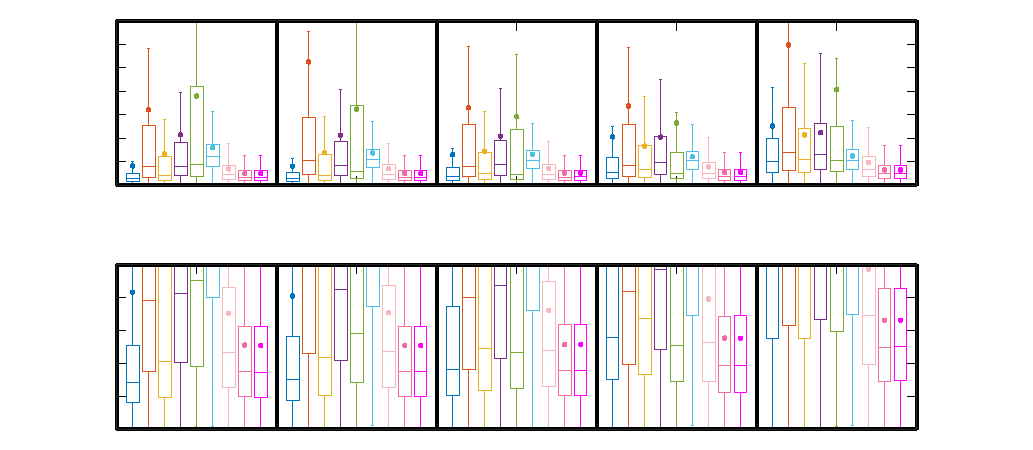
\includegraphics{./figures/parts/02/chapters/04/sections/05/boxplots_pose_errors_sm5}}%
    \gplfronttext
  \end{picture}%
\endgroup
